%------------ SECTION %------------
% Victor
\section{Análise da rede elétrica nacional}

A produção de energia elétrica em Portugal é aberta ao livre mercado e concorrência, tendo dois regimes legais, a saber \cite{REN-site}:
\begin{itemize}
\item Produção em regime ordinário (PRO): relativo à produção de eletricidade a partir de fontes não renováveis ou em grandes centrais hídricas;
\item Produção em regime especial (PRE): relativo à produção de eletricidade a partir de fontes renováveis ou cogeração.
\end{itemize}

O transporte, ou transmissão, da energia elétrica é realizada através da Rede Nacional de Transporte
%\sigla[Rede Nacional de Transporte]{RNT}% 
, a saber a rede de 150 a 400 kV, através de concessão pelo Estado Português em regime de serviço público e exclusividade à Redes Energéticas Nacionais %\sigla[Redes Energéticas Nacionais]{REN}%
. Tal concessão inclui planeamento, construção, operação e manutenção da RNT \cite{REN-site}.

A rede de distribuição é efetivada através da exploração da Rede Nacional de Distribuição %\sigla[Rede Nacional de Distribuição]{RND}%
. A rede de baixa tensão é operada através de contratos estabelecidos entre os municípios e as distribuidoras \cite{REN-site}.

Em relação ao consumo, no Portugal Continental há 6,1 milhões de consumidores em maioria na baixa tensão, 23 500 na média tensão, 350 na alta tensão e muito alta tensão, até 400 kV. O consumidor é livre para escolher o seu comercializador de energia elétrica \cite{REN-site}.

O Sistema Elétrico Nacional %\sigla[Sistema Elétrico Nacional]{SEN}
, ilustrado de forma simplificada na Figura \ref{fig:Organizacao_SEP_PT}, é composto pela parte da produção: PRO, PRE e importação; pela parte do transporte: RNT; pela parte de comercialização: Comercializador Liberalizado e Comercializador de Último Recurso %\sigla[Comercializador de Último Recurso]{CUR}%
; e por fim, pela parcela da distribuição: clientes do mercado liberalizado e do CUR. Os comercializadores liberalizados e de último recurso estão enquadrados no Mercado Organizado. A Entidade Reguladora dos Serviços Energéticos %\sigla[Entidade Reguladora dos Serviços Energéticos]{ERSE}%
é quem estabelece as tarifas pagas pelos comercializadores para acenderem à RNT e RND. Todo esse sistema está sob o enquadramento legislativo e regulamentar da Direção Geral de Energia e Geologia %\sigla[Direção Geral de Energia e Geologia]{DGGE}%
\cite{gil2010analise}.

\begin{figure}[H]
	\centering
	\captionsetup{width=\textwidth, font=footnotesize, textfont=bf}	
	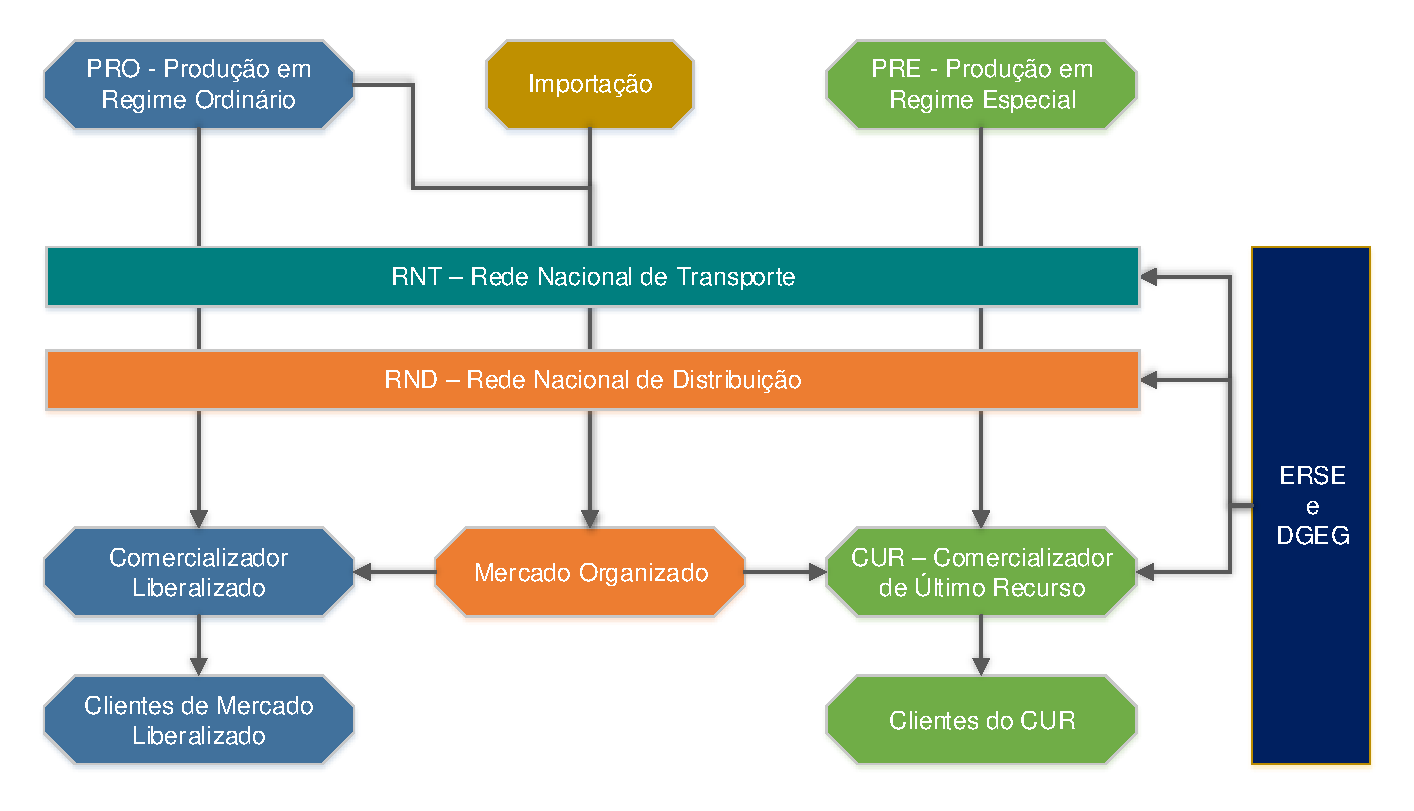
\includegraphics[width=\textwidth]{img/Organizacao_SEP_PT.pdf}
	\caption{Esquema simplificado da Organização do Sistema Elétrico Nacional.}
	\vspace{-3.5mm}
	\caption*{Fonte: \cite{gil2010analise}}
	\label{fig:Organizacao_SEP_PT}
\end{figure}

%------------ SECTION %------------
% Carlos
\section{Caracterização das centrais}

% Localização; 
% potência Instalada;
% Especificações

%----------- SECTION %------------
% Carlos
\section{Caracterização da RNT} 

% Capacidade; 
% especificações


%------------ SECTION %------------
% Callebe
\section{Perfil de produção nacional} 

Segunda a \citeonline[p.~5]{e2p}, desde 2000 as fontes renováveis apresentaram um crescimento continuo na matriz energética portuguesa, sobre tudo a geração eólica. Este franco crescimento foi proveniente de uma política europeia e nacional que tem como objetivo a melhoria da segurança de abastecimento, redução da dependência energética e redução dos impactos ambientais do sistema elétrico.  

Como resultado da política energética portuguesa, em 2016  57\% da produção de energia elétrica em Portugal se deu através de fontes renováveis. Face ao ano anterior as fontes renováveis aumentaram 10\% na participação da produção \cite[p.~8]{REN}. O aumento da produção renovável e 2016 deve-se, em parte, da entrada da central hidroelétrica de Frades II, equipada com 780 MW, e do crescimento em 236 MW de potência instalada em parques eólicos portugueses. Seguindo assim uma tendência de crescimento desde 2014, o que pode ser verificada através das estatísticas diária disponibilizadas pela \citeonline{REN-site}.  Em 2016 a geração hidráulica representou 28\% da produção nacional, enquanto a geração eólica representou 22\%, a biomassa representou 5\% e a solar contribuiu com 1\%.

Um fato importante sobre a geração renovável em 2016 é que devido a sua grande participação na produção de energia houve uma redução no preço médio do MWh no mercado ibérico de eletricidade, valor este que esteve situado em 39,4 \euro/MWh \cite[p.~4]{apren}. Comparado ao ano de 2015, quando o custo médio esteve em 50,4 \euro/MWh e a contribuição das renováveis para a matriz energética foi de 48 \%, nota-se uma relação entre o custo \euro/MWh e a  produção renovável. A Figura \ref{fig:CorrelacaoPrecoMercadoProducaoRenovavel} deixa mais explicita esta relação entre o anos de 2015 e 2016.

\begin{figure}[H]
	\centering
	\captionsetup{width=0.85\textwidth, font=footnotesize, textfont=bf}
	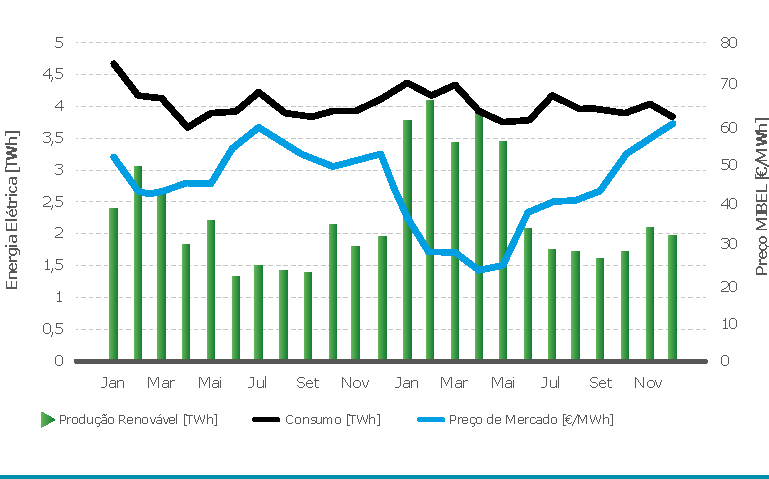
\includegraphics[width=0.8\linewidth]{img/CorrelacaoPrecoMercadoProducaoRenovavel.pdf}
	\caption{Correlação entre o Preço de Mercado e a Produção Renovável (2015-16) }
	\vspace{-3.5mm}
	\caption*{Fonte: \citeonline[p.~10]{apren}}
	\label{fig:CorrelacaoPrecoMercadoProducaoRenovavel}
\end{figure}

Já pelo lado das fontes não renováveis a geração por termoelétricas a carvão e a gás natural ambas representaram, em 2016, 21\% da produção. Face ao ano anterior a produção a carvão sofreu uma queda de 14\%, já a produção a gás natural cresceu 18\% \cite[p.~8]{REN}. Os dados a produção nacional em 2016 estão dispostas Gráfico \ref{fig:ReparticaoDaProducao}, e para fins de comparação está a Tabela \ref{tab:producao20152016}.

\begin{figure}[H]
	\centering
	\captionsetup{width=0.7\textwidth, font=footnotesize, textfont=bf}
	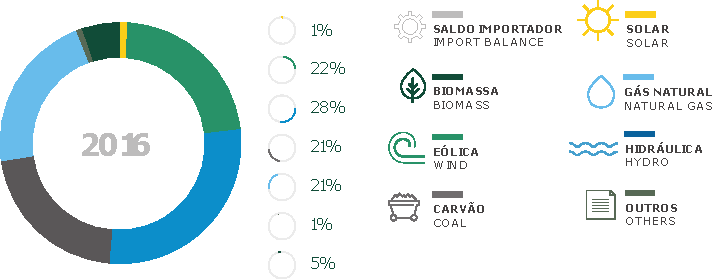
\includegraphics[width=0.7\linewidth]{img/ReparticaoDaProducao2016.pdf}
	\caption{Repartição da Produção}
	\vspace{-3.5mm}
	\caption*{Fonte: \citeonline[p.~8]{REN}}
	\label{fig:ReparticaoDaProducao}
\end{figure}

\begin{table}[H]
	\centering
	\captionsetup{width=0.74\textwidth, font=footnotesize, textfont=bf}
    \begin{tabular}{|l|c|c|c|}
    \rowcolor[HTML]{000000}
    {\color[HTML]{FFFFFF} Geração} & {\color[HTML]{FFFFFF} 2015} & {\color[HTML]{FFFFFF} 2016}   & {\color[HTML]{FFFFFF} Variação(\%) }  \\
    Hídrica                 & 8.453  & 15.413 & 82           \\
    Eólica                  & 11.334 & 12.188 & 8            \\
    Biomassa                & 2.618  & 2.687  & 3            \\
    Solar                   & 760    &  781   & 3            \\
    Carvão                  & 13.677 & 11.698 & -14          \\
    Gás Natural             & 9.807  & 11.571 & 18           \\
    Produção por Bombagem   & 1.160  & 1.217  & 5            \\
    Saldo Importador        & 2.266  & -5.085 & -            \\ \hline
    Produção Não Renovável  & 23.840 & 23.587 & -1           \\ \hline
    Produção Renovável      & 23.165 & 31.069 & 34           \\ \hline
    Produção Total          & 48.165 & 55.873 & 16           \\ \hline
    \end{tabular}
    \caption{Produção Nacional 2015/2016}
    \vspace{-3.5mm}
	\caption*{Fonte: \citeonline[p.~10]{REN}}
    \label{tab:producao20152016}
\end{table}



%------------ SECTION %------------
% Callebe
\section{Perfil de Consumo Nacional}

Em relação ao consumo nacional Portugal vem apresentando um crescimento continuo desde 2012, e se consolida em 2016 com um total de  49,3 TWh, um consumo menor apenas 5,6\% do máximo histórico registrado em 2010. Tal crescimento no consumo tem relação direta com o crescimento social e económico do pais, e indica uma tendência para os próximos anos\cite[p.~6]{REN}. 

O gráfico da Figura \ref{fig:SatisfacaoDoConsumo} apresenta a relação dos máximos de consumo e produção registrados desde 2012. Este gráfico torna claro a evolução dos picos de produção sobre os máximos de consumo ao longo dos anos. A relação entre picos de produção e consumo representam uma margem que assegura atendimento da carga mesmo nos dias de maior pico.

\begin{figure}[H]
	\centering
	\captionsetup{width=0.7\textwidth, font=footnotesize, textfont=bf}	
	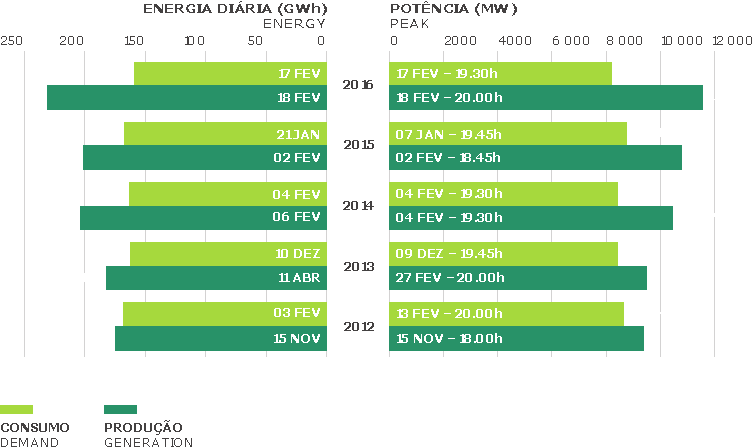
\includegraphics[width=0.7\linewidth]{img/ConsumoEProducaoMaximosAnuais.pdf}
	\caption{Consumo e Produção Máximos Anuais}
	\vspace{-3.5mm}
	\caption*{Fonte: \citeonline{REN}}
	\label{fig:SatisfacaoDoConsumo}
\end{figure}

Em 2016 o dia de maior pico no consumo ocorreu no dia 17 de fevereiro, já em 2015 o dia de maior pico no consumo foi registrado no dia 7 de janeiro. Mas apenas em  2016, mesmo no horário de pico todo o consumo foi atendido pela geração nacional, ou seja não houve saldo importador. Como pode ser visto na Figura \ref{fig:ConsumoDiaDePontaAnual} \cite{apren}.

\begin{figure}[H]
	\centering
	\captionsetup{width=0.7\textwidth, font=footnotesize, textfont=bf}	
	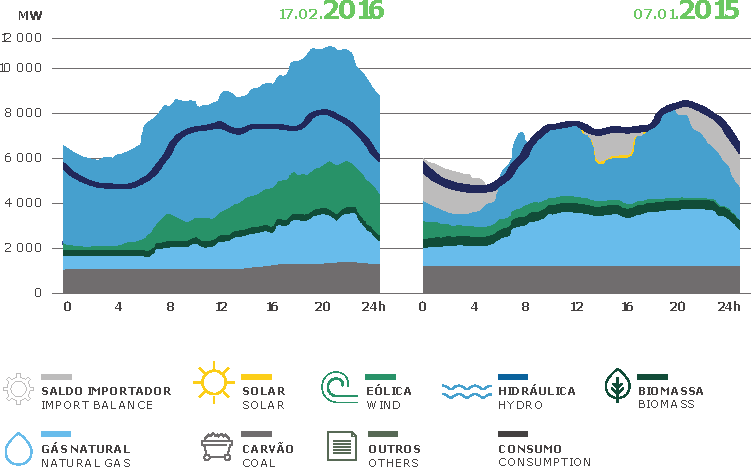
\includegraphics[width=0.7\linewidth]{img/ConsumoDiaDePontaAnual.pdf}
	\caption{Diagrama de Consumo no Dia de Ponta Anual}
	\vspace{-3.5mm}
	\caption*{Fonte: \citeonline{REN}}
	\label{fig:ConsumoDiaDePontaAnual}
\end{figure}

Em 2016 houve um total de  1130 horas em que a eletricidade renovável por si só, foi suficiente para suprir as necessidades elétricas de Portugal. Ainda neste ano, entre as 6:45h do dia 7 e 17:45h do dia 11 de maio, foi registrado um período de 107 horas consecutivas em que a produção renovável excedeu o consumo elétrico \cite{apren}. Estes fato que demonstra que mesmo com o aumento do consumo, a geração renovável e supera o consumo em vários períodos relevantes. 

Segundo a \citeonline{apren} em 2016 houve um importante marco do saldo exportador de 5,1 TWh, que constitui uma inversão na tendência de importação apresentada nos últimos 15 anos. O gráfico da Figura \ref{fig:SatisfacaoDoConsumo} trás um comparativo da satisfação do consumo anual entre 2007 e 2016. 

\vspace{5.5mm}

\begin{figure}[H]
	\centering
	\captionsetup{width=0.7\textwidth, font=footnotesize, textfont=bf}	
	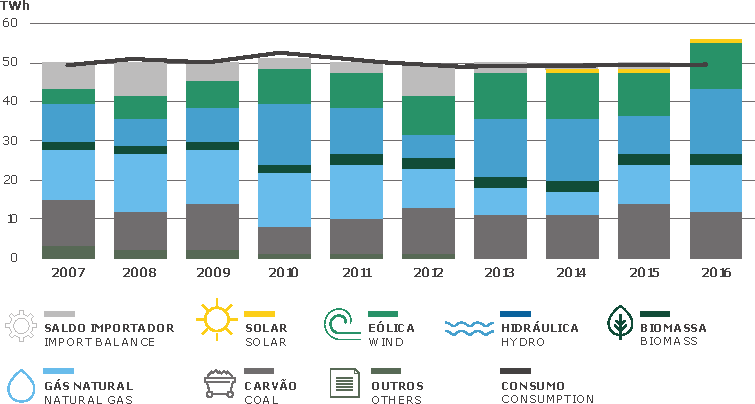
\includegraphics[width=0.7\linewidth]{img/SatisfacaoDoConsumo.pdf}
	\caption{Satisfação do Consumo}
	\vspace{-3.5mm}
	\caption*{Fonte: \citeonline[p.~10]{REN}}
	\label{fig:SatisfacaoDoConsumo}
\end{figure}




